\chapter{Aplikacja mobilna} % (fold)
\label{cha:mobileapp}

\paragraph{} % (fold)
\label{par:}
Aplikacja mobilna jest integralną częścią całego systemu do wspierania treningów areobowych. Jej zadaniem jest pobieranie informacji o przebytej trasie za pomocą odbiornika GPS, obliczanie dystansu i czasu trwania treningu, przetrzymywanie informacji w bazie danych oraz synchronizacja rekordów z apikacją internetową. 
% paragraph  (end)

\section{Architektura systemu} % (fold)
\label{sec:architektura_system}

% section architektura_system (end)
\paragraph{} % (fold)
\label{par:}
Aplikacja została napisana w języku Java i działa na mobilnej platformie Android w wersji 4.0.3. Najważniejszą częścia programów napisanych na system Android jest \textit{Aktywność (ang. Activity)}, charakteryzująca się określonym cyklem życia. Sposób w jaki zarządza się cyklem życia aplikacji, uruchamia odpowiednie zdarzenia w określonych momentach i zachowanie aktywności ma fundamentalny wpływ na działanie całej aplikacji.

\subsection{Aktywności} % (fold)
\label{sub:aktywno_ci}

% subsection aktywno_ci (end)
\paragraph{} % (fold)
\label{par:}
Aktywności wyróżniają się czterema stanami:
\begin{itemize}
	\item aktywna (ang. active) lub chodząca (ang. running) - gdy aktywność znajduje się w warstwie szczytowej aplikacji,
	\item wstrzymana (ang. paused) - gdy aktywność jest widoczna, ale nie znajduje się na pierwszym planie. W tym stanie może zostać zakończona przez system, w przypadku braku pamięci,
	\item zatrzymana (ang. stopped) - gdy aktywność zostanie zasłonięta przez inna aktywność. W tym stanie system przechowuje pełną informację na temat aktywności, lecz nie jest widoczna dla użytkownika,
	\item gdy aplikacja jest w stanie wstrzymania lub zatrzymania, może zostać usunięta z pamięci systemu. W momencie ponownego uruchomienia, aktywność będzie musiała być stworzona od początku.
\end{itemize}

\paragraph{} 
Pełny cykl życia aktywności został przedstawiony na Rysunku \ref{fig:activity_lifecycle}

\begin{figure}[ht]
	\centering
		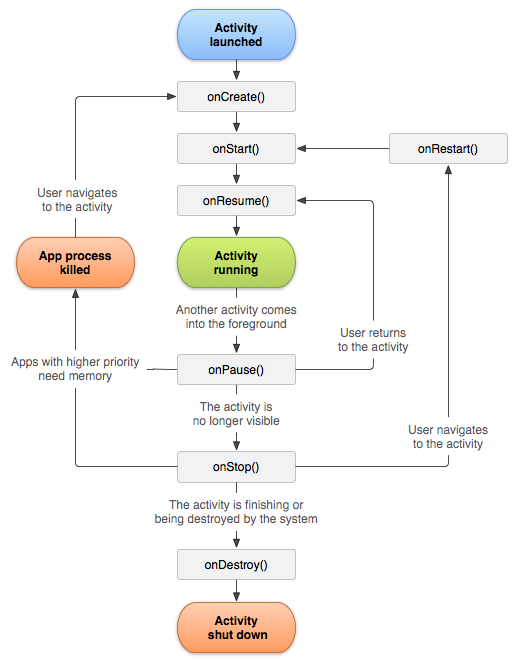
\includegraphics[width=0.7\linewidth]{assets/activity_lifecycle.png}
		\caption{Pełny cykl życia aktywności}
	\label{fig:activity_lifecycle}
\end{figure}

\subsection{Moduł GPS} % (fold)
\label{sub:modu_gps}

% subsection modu_gps (end)
\paragraph{} % (fold)
\label{par:}
Obsługa modułu GPS polega na zaimplementowaniu interfejsów odpowiedzialnych za zczytywanie informacji (\textit{LocationListener}) na temat położenia i badanie stanu odbiornika GPS (\textit{GpsStatusListener}). Oba interfejsy są uruchamiane w zdarzeniu \textit{onCreate()} głównej aktywności.
 
\newpage
\subsection{Baza danych} % (fold)
\label{sub:baza_danych}
\paragraph{} % (fold)
\label{par:}

% paragraph  (end)
Informacje na temat treningów przechowywane są w bazie danych SQLite \footnote{SQLLite - Sekcja \ref{sub:sqlite}}. Model bazy danych (Rysunek \ref{fig:sqlite-model}) stanowią dwie tabele: \textit{Workout} i \textit{WorkoutDetails}. Pierwsza z nich służy do przechowywania podstawowych informacji o treningu: początek, koniec, czas trwania, dystans. W drugiej tabeli natomiast przechowywane są współrzędne geograficzne zczytane z GPS.
% subsection baza_danych (end)
\begin{figure}[ht]
	\centering
		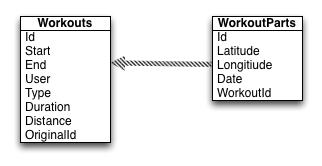
\includegraphics[width=0.6\linewidth]{assets/sql_schema.png}
		\caption{Schemat bazy danych w aplikacji mobilnej}
	\label{fig:sqlite-model}
\end{figure}

\subsection{Autoryzacja} % (fold)
\label{sub:}
\paragraph{} % (fold)
\label{par:}
% paragraph  (end)
Po wprowadzeniu nazwy użytkownika i hasła w formularzu na aktywności Login, wysłane zostaje żądanie autoryzacji do REST API. Po pozytywnej weryfikacji danych zwrócona zostaje odpowiedź o statusie HTTP 200 wraz z tokenem, służącym do dalszej autoryzacji aplikacji. Zweryfikowane dane użytkownika (login i hasło) przechowywane są w \textit{SharedPreferences}. Szczegółowy opis autoryzacji znajduje się w sekcji \ref{sub:autoryzacja}.

\newpage
\subsection{Wielojęzykowość} % (fold)
\label{sub:wieloj_zykow_}
\paragraph{} % (fold)
\label{par:}

% paragraph  (end)
Podobnie jak strona internetowa, aplikacja mobilna została dostosowana do wielojęzykowości, dzięki popularnemu w środowisku android systemowi zasobów.
% subsection wieloj_zykow_ (end)

\subsection{Wyświetlanie mapy} % (fold)
\label{sub:wy_wietlanie_mapy}
\paragraph{} % (fold)


W celu wyświetlenia przebytej trasy w aplikacji mobilnej wykorzystane zostało \textit{Google Maps Android API}. Pozwala ono na pobranie z serwisu Google mapy o wskazanej pozycji i przybliżeniu, a także na rysowaniu lini pomiędzy punktami na jednej z jej warstw. 

\paragraph{}
Aby wyznaczyć środek wyświetlanego obszaru, trzeba znaleźć cztery wartości: maksymalną i minimalną długość i szerokość. Punkt środka mapy wyznacza się z następującego wzoru:

\begin{equation}
	CenterLatitude = \frac{MaxLatitude + MinLatitude}{2}
\end{equation}

\begin{equation}
		CenterLongitude = \frac{MaxLongitiude + MinLongitiude}{2}
\end{equation}

\paragraph{} % (fold)
\label{par:}
Następnym etapem jest pobranie z bazy danych współrzędnych zarejestrowanych punktów i połączenie ich za pomocą linii.
% paragraph  (end)



\begin{figure}[h]
\begin{center}$
\begin{array}{cc}
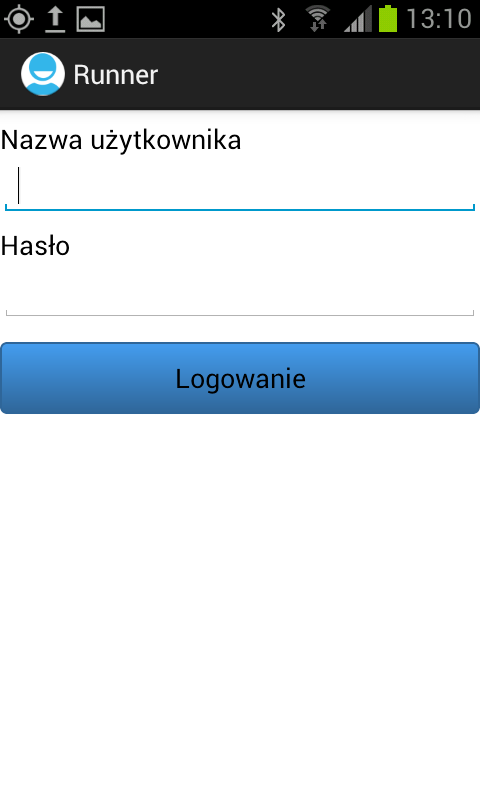
\includegraphics[width=0.4\linewidth]{assets/and1.png}&
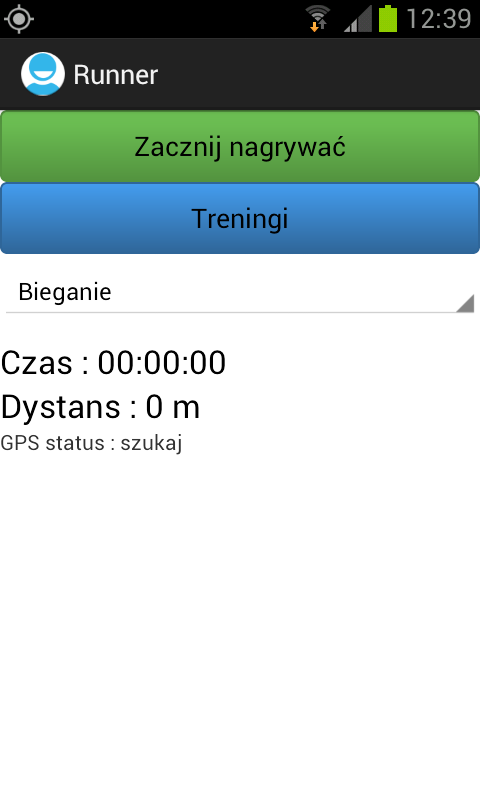
\includegraphics[width=0.4\linewidth]{assets/and2.png}
\end{array}$
\end{center}
\caption{Po lewej ekran logowania, po prawej ekran główny apliakcji}
\end{figure}

\begin{figure}[h]
\begin{center}$
\begin{array}{cc}
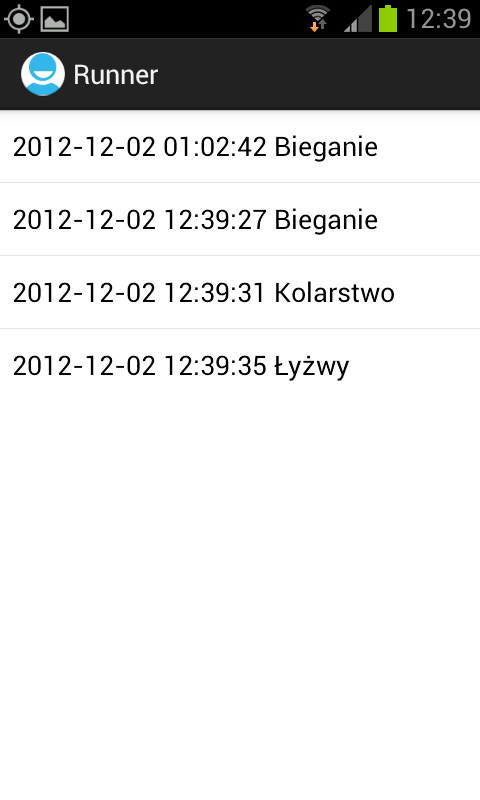
\includegraphics[width=0.4\linewidth]{assets/and3.png}&
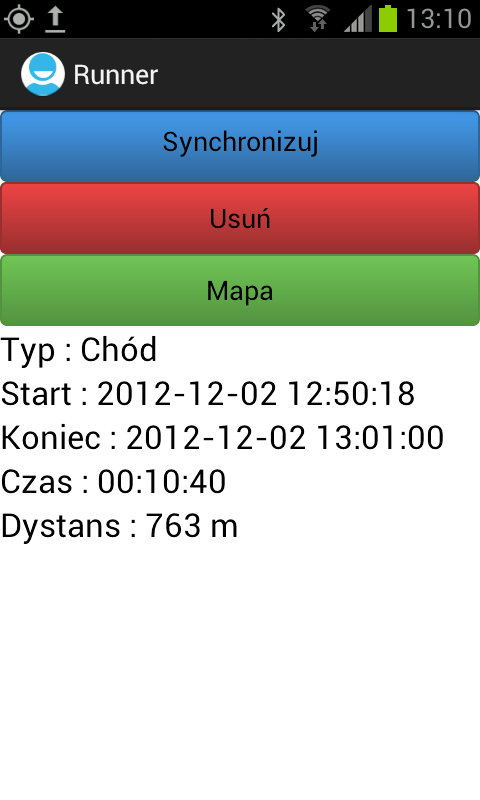
\includegraphics[width=0.4\linewidth]{assets/and4.png}
\end{array}$
\end{center}
\caption{Po lewej lista treningów, po prawej szczegółowy widok treningu}
\end{figure}


\begin{figure}[ht]
	\centering
		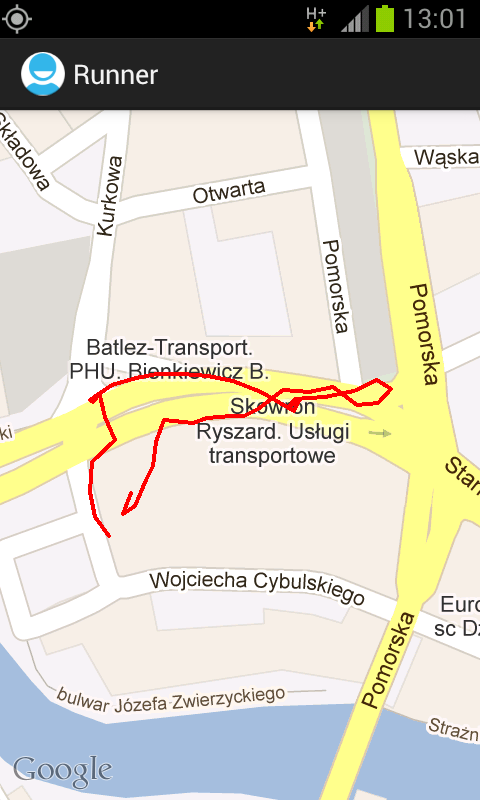
\includegraphics[width=0.4\linewidth]{assets/and5.png}
	\caption{Widok zaznaczonej na mapie trasy}
	\label{fig:and5}
\end{figure}
